\documentclass[tikz,border=2pt]{standalone}
\usetikzlibrary{positioning}
\begin{document}
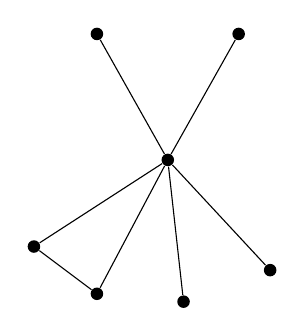
\begin{tikzpicture}[vertex/.style={circle,fill,inner sep=1.6pt}]
    \node[vertex] (c)  at (0,0)      {};
    \node[vertex] (t1) at (-0.9,1.6) {};
    \node[vertex] (t2) at (0.9,1.6)  {};
    \node[vertex] (b1) at (-1.7,-1.1) {};
    \node[vertex] (b2) at (-0.9,-1.7) {};
    \node[vertex] (b3) at (0.2,-1.8) {};
    \node[vertex] (b4) at (1.3,-1.4) {};

    \draw (c) -- (t1);
    \draw (c) -- (t2);
    \draw (c) -- (b1);
    \draw (b1) -- (b2);
    \draw (b2) -- (c);
    \draw (c) -- (b3);
    \draw (c) -- (b4);
\end{tikzpicture}
\end{document}
